\documentclass[tikz,border=20pt]{standalone}
\usepackage{tikz}
\usepackage{amsmath}
\usetikzlibrary{arrows.meta,positioning,shapes}

\begin{document}
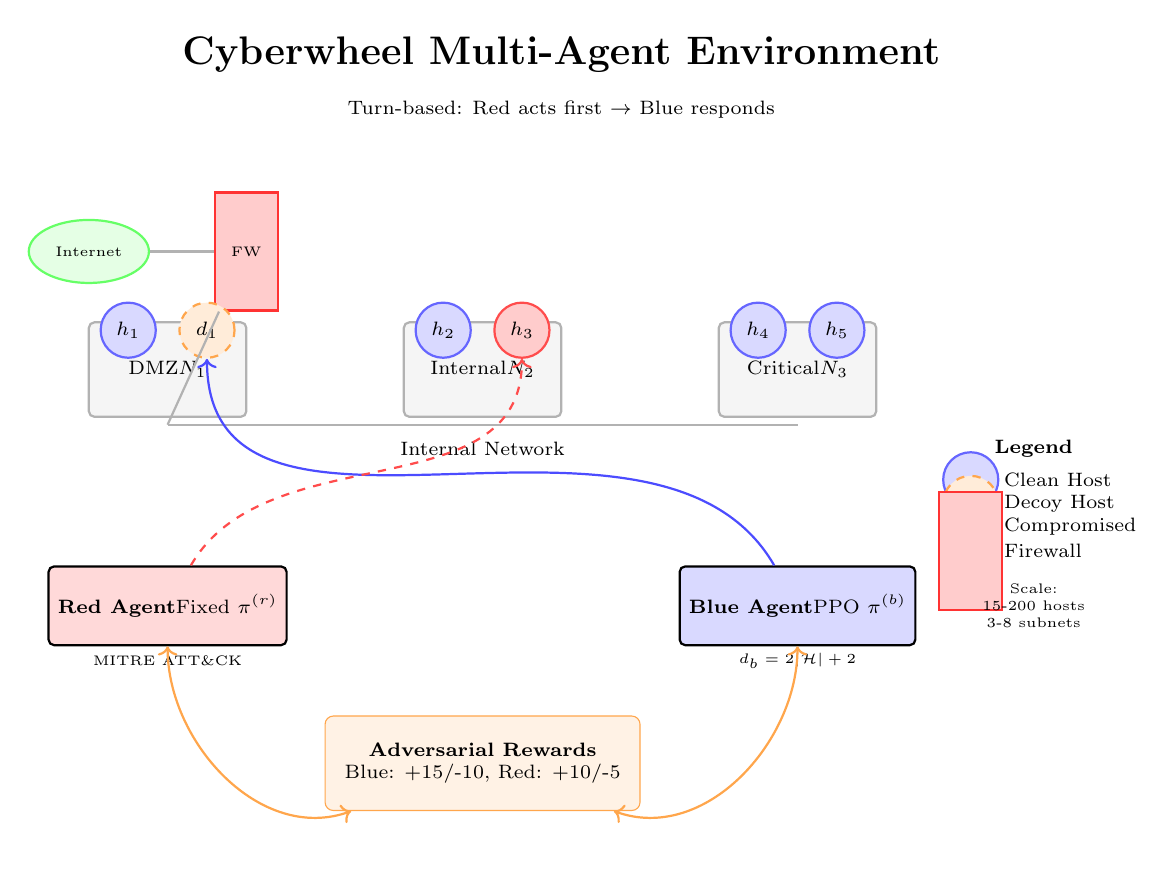
\begin{tikzpicture}[
    host/.style={circle, draw=blue!60, fill=blue!15, minimum size=7mm, font=\scriptsize, thick},
    decoy/.style={circle, draw=orange!70, fill=orange!15, minimum size=7mm, font=\scriptsize, thick, dashed},
    compromised/.style={circle, draw=red!70, fill=red!20, minimum size=7mm, font=\scriptsize, thick},
    subnet/.style={rectangle, draw=gray!60, fill=gray!8, minimum width=20mm, minimum height=12mm, font=\scriptsize, thick, rounded corners=2pt},
    agent/.style={rectangle, draw=black, fill=yellow!15, minimum width=18mm, minimum height=10mm, font=\scriptsize, thick, rounded corners=2pt},
    firewall/.style={rectangle, draw=red!80, fill=red!20, minimum width=8mm, minimum height=15mm, font=\tiny, thick},
    internet/.style={ellipse, draw=green!60, fill=green!10, minimum width=15mm, minimum height=8mm, font=\tiny, thick}
]

% Title with more space
\node[font=\Large\bfseries] at (0, 8.5) {Cyberwheel Multi-Agent Environment};

% Internet - top left
\node[internet] (internet) at (-6, 6) {Internet};

% Firewall - gateway
\node[firewall] (firewall) at (-4, 6) {FW};

% Network subnets - more spaced out
\node[subnet] (subnet1) at (-5, 4.5) {DMZ\\$N_1$};
\node[subnet] (subnet2) at (-1, 4.5) {Internal\\$N_2$};  
\node[subnet] (subnet3) at (3, 4.5) {Critical\\$N_3$};

% Hosts - positioned above subnets to avoid overlap
\node[host] (h1) at (-5.5, 5) {$h_1$};
\node[decoy] (d1) at (-4.5, 5) {$d_1$};

\node[host] (h2) at (-1.5, 5) {$h_2$};
\node[compromised] (h3) at (-0.5, 5) {$h_3$};

\node[host] (h4) at (2.5, 5) {$h_4$};
\node[host] (h5) at (3.5, 5) {$h_5$};

% Network connections
\draw[thick, gray!60] (internet) -- (firewall);
\draw[thick, gray!60] (firewall) -- (-5, 3.8);
\draw[thick, gray!60] (-5, 3.8) -- (-1, 3.8) -- (3, 3.8);
\node[font=\scriptsize] at (-1, 3.5) {Internal Network};

% Agents - more separated
\node[agent, fill=red!15] (red) at (-5, 1.5) {\textbf{Red Agent}\\Fixed $\pi^{(r)}$};
\node[agent, fill=blue!15] (blue) at (3, 1.5) {\textbf{Blue Agent}\\PPO $\pi^{(b)}$};

% Key interactions - cleaner paths to avoid subnet overlap
\draw[->, thick, blue!70] (blue) to[out=120, in=270] (d1) node[near end, right, font=\tiny] {deploy};
\draw[->, thick, red!70, dashed] (red) to[out=60, in=270] (h3) node[near end, left, font=\tiny] {attack};

% Essential state info
\node[font=\tiny] at (-5, 0.8) {MITRE ATT\&CK};
\node[font=\tiny] at (3, 0.8) {$d_b = 2|\mathcal{H}| + 2$};

% Reward system - larger box to fit text properly
\node[rectangle, draw=orange!70, fill=orange!10, minimum width=40mm, minimum height=12mm, rounded corners=3pt] at (-1, -0.5) (reward) {};
\node[font=\scriptsize, align=center] at (reward.center) {\textbf{Adversarial Rewards}\\Blue: +15/-10, Red: +10/-5};

% Reward connections - cleaner paths
\draw[<->, orange!70, thick] (red) to[out=270, in=200] (reward);
\draw[<->, orange!70, thick] (blue) to[out=270, in=340] (reward);

% Turn sequence
\node[font=\scriptsize] at (0, 7.8) {Turn-based: Red acts first $\rightarrow$ Blue responds};

% Legend - moved further right with more space
\node[font=\scriptsize] at (6, 3.5) {\textbf{Legend}};
\node[host] at (5.2, 3.1) {}; \node[right, font=\scriptsize] at (5.5, 3.1) {Clean Host};
\node[decoy] at (5.2, 2.8) {}; \node[right, font=\scriptsize] at (5.5, 2.8) {Decoy Host};
\node[compromised] at (5.2, 2.5) {}; \node[right, font=\scriptsize] at (5.5, 2.5) {Compromised};
\node[firewall] at (5.2, 2.2) {}; \node[right, font=\scriptsize] at (5.5, 2.2) {Firewall};

% Environment info
\node[font=\tiny, align=center] at (6, 1.5) {Scale:\\15-200 hosts\\3-8 subnets};

\end{tikzpicture}
\end{document}





\documentclass[tikz,border=15pt]{standalone}
\usepackage{tikz}
\usepackage{amsmath}
\usetikzlibrary{arrows.meta,positioning,shapes}

\begin{document}
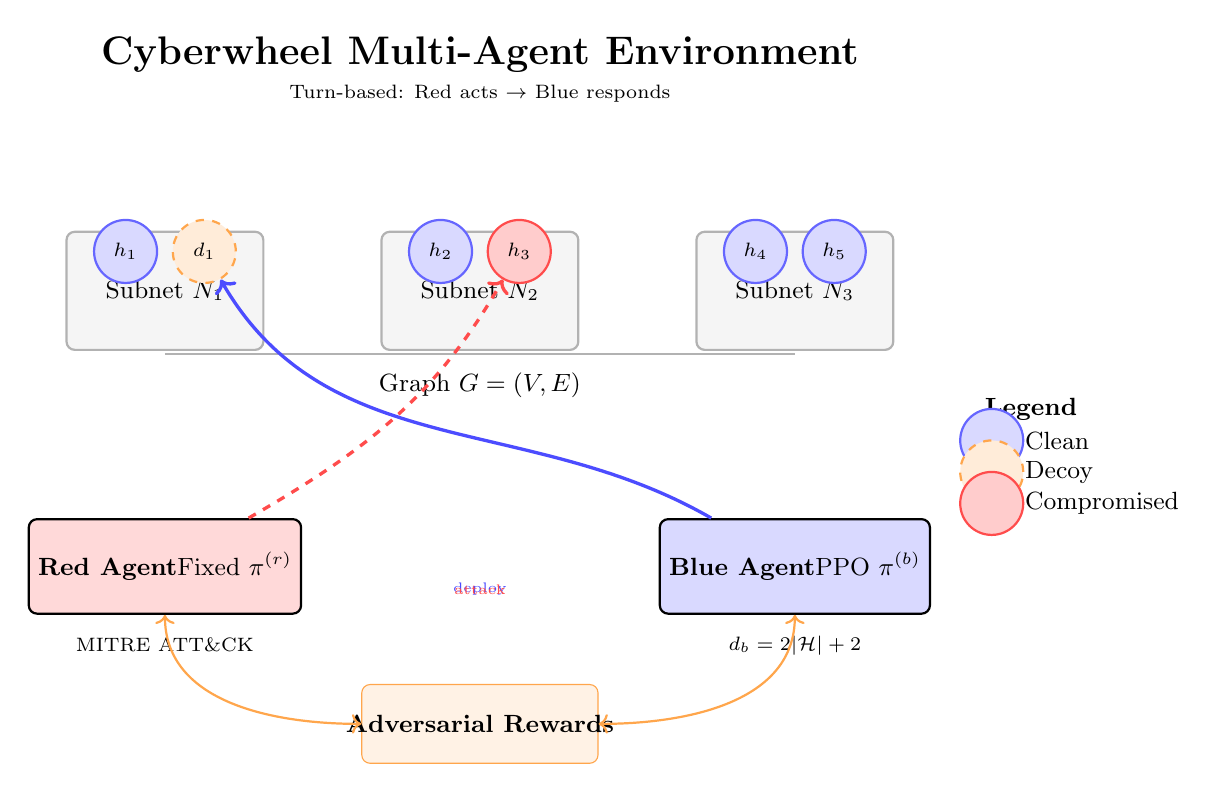
\begin{tikzpicture}[
    host/.style={circle, draw=blue!60, fill=blue!15, minimum size=8mm, font=\scriptsize, thick},
    decoy/.style={circle, draw=orange!70, fill=orange!15, minimum size=8mm, font=\scriptsize, thick, dashed},
    compromised/.style={circle, draw=red!70, fill=red!20, minimum size=8mm, font=\scriptsize, thick},
    subnet/.style={rectangle, draw=gray!60, fill=gray!8, minimum width=25mm, minimum height=15mm, font=\small, thick, rounded corners=3pt},
    agent/.style={rectangle, draw=black, fill=yellow!15, minimum width=20mm, minimum height=12mm, font=\small, thick, rounded corners=3pt}
]

% Title
\node[font=\Large\bfseries] at (0, 7) {Cyberwheel Multi-Agent Environment};

% Network subnets  
\node[subnet] (subnet1) at (-4, 4) {Subnet $N_1$};
\node[subnet] (subnet2) at (0, 4) {Subnet $N_2$};  
\node[subnet] (subnet3) at (4, 4) {Subnet $N_3$};

% Hosts
\node[host] (h1) at (-4.5, 4.5) {$h_1$};
\node[decoy] (d1) at (-3.5, 4.5) {$d_1$};

\node[host] (h2) at (-0.5, 4.5) {$h_2$};
\node[compromised] (h3) at (0.5, 4.5) {$h_3$};

\node[host] (h4) at (3.5, 4.5) {$h_4$};
\node[host] (h5) at (4.5, 4.5) {$h_5$};

% Network backbone
\draw[gray!60, thick] (-4, 3.2) -- (0, 3.2) -- (4, 3.2);
\node[font=\small] at (0, 2.8) {Graph $G = (V, E)$};

% Agents
\node[agent, fill=red!15] (red) at (-4, 0.5) {\textbf{Red Agent}\\Fixed $\pi^{(r)}$};
\node[agent, fill=blue!15] (blue) at (4, 0.5) {\textbf{Blue Agent}\\PPO $\pi^{(b)}$};

% Key interactions
\draw[->, very thick, blue!70] (blue) to[out=150, in=300] (d1) node[midway, above, font=\tiny] {deploy};
\draw[->, very thick, red!70, dashed] (red) to[out=30, in=240] (h3) node[midway, above, font=\tiny] {attack};

% Essential state info - minimal
\node[font=\scriptsize] at (-4, -0.5) {MITRE ATT\&CK};
\node[font=\scriptsize] at (4, -0.5) {$d_b = 2|\mathcal{H}| + 2$};

% Reward system
\node[rectangle, draw=orange!70, fill=orange!10, minimum width=30mm, minimum height=10mm, rounded corners=3pt] at (0, -1.5) (reward) {};
\node[font=\small] at (reward.center) {\textbf{Adversarial Rewards}};

% Reward connections
\draw[<->, orange!70, thick] (red) to[out=270, in=180] (reward);
\draw[<->, orange!70, thick] (blue) to[out=270, in=0] (reward);

% Turn sequence - minimal text
\node[font=\scriptsize] at (0, 6.5) {Turn-based: Red acts $\rightarrow$ Blue responds};

% Legend - far right
\node[font=\small] at (7, 2.5) {\textbf{Legend}};
\node[host] at (6.5, 2.1) {}; \node[right, font=\small] at (6.8, 2.1) {Clean};
\node[decoy] at (6.5, 1.7) {}; \node[right, font=\small] at (6.8, 1.7) {Decoy};
\node[compromised] at (6.5, 1.3) {}; \node[right, font=\small] at (6.8, 1.3) {Compromised};

\end{tikzpicture}
\end{document}